\documentclass{beamer}
\usetheme{Madrid}
\title{Neural Implicit Flow (NIF)}
\author{Christian Beneke}
\date{28.11.2024}

\begin{document}

\frame{\titlepage}

\begin{frame}{Problem Statement}
\begin{itemize}
    \item Spatio-temporal data modeled by PDEs is computationally challenging.
    \item Current reduction methods (SVD, CAE) fail with variable geometry or adaptive meshing.
    \item Need for a scalable, mesh-agnostic approach for real-time engineering applications.
    \item Examples: Sea surface temperature modeling, turbulence modeling, sparse sensing.
\end{itemize}
\end{frame}

\begin{frame}{New Approach: Neural Implicit Flow (NIF)}
\begin{itemize}
    \item Combines two neural networks:
    \begin{itemize}
        \item \textbf{ShapeNet:} Encodes spatial complexity mesh-agnostically.
        \item \textbf{ParameterNet:} Models temporal and parametric dependencies.
    \end{itemize}
    \item Provides efficient, nonlinear dimensionality reduction and interpretable representations.
\end{itemize}
\begin{figure}
    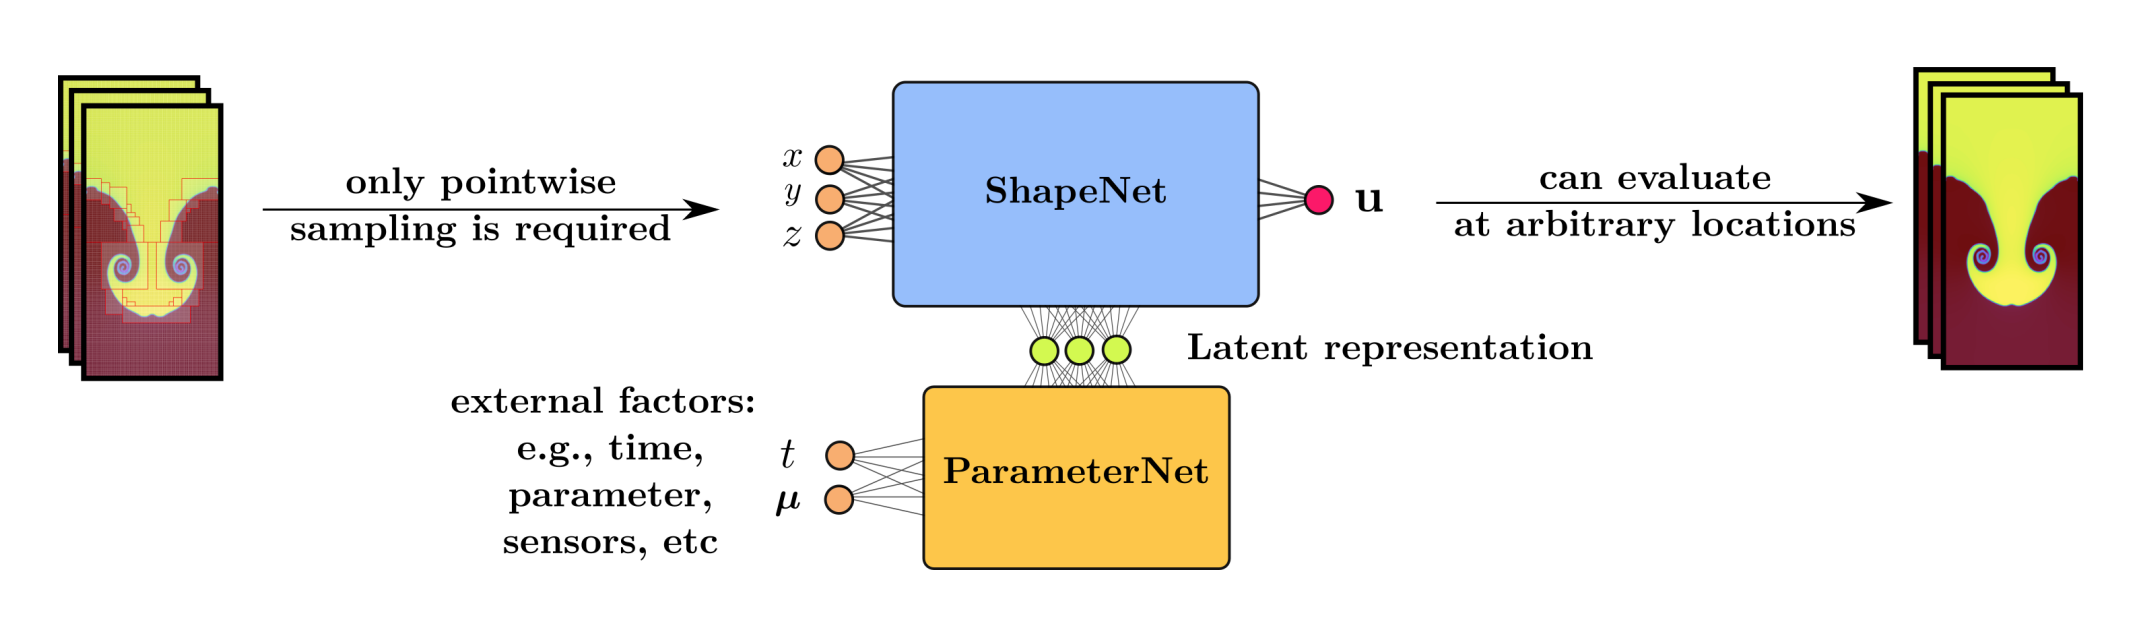
\includegraphics[width=0.6\linewidth]{hypernetwork_diagram.png}
    \caption{NIF Hypernetwork Architecture}
\end{figure}
\end{frame}

\begin{frame}{My Contributions}
\begin{itemize}
    \item Performance tuning of the provided implementation.
    \item Re-Evaluation of the results
    \begin{itemize}
        \item 40\% better generalization performance
        \item Scalable to complex spatio-temporal datasets
    \end{itemize}
\end{itemize}
\end{frame}

\begin{frame}{My Contributions - Performance tuning}
\begin{itemize}
    \item Performance tuning of the provided implementation.
    \begin{itemize}
        \item Port from Tensorflow to PyTorch
        \item Implementation using upstream SIREN
        \item Improving parallelism in learning phase
    \end{itemize}
\end{itemize}
\end{frame}

\begin{frame}{My Contributions - Result Re-Evaluation}
\begin{itemize}
    \item Re-Evaluation of results - with focus on chaotic systems
    \begin{itemize}
        \item Comparison to other Hypernetworks / LoRA / etc
        \item Comparing the existing results using own implementation
    \end{itemize}
\end{itemize}
\end{frame}

\end{document}
